
\chapter{Development} \label{development}

In this chapter, the software development process will be covered, including the adopted strategy and tools used in the development of the web based platform. The different modules, as well as the data model used for project, dataset and user management will also be explained, covering the encryption process for secure data storage in the database.


\section{Development Strategy and Tools}

A web based platform with features covering the main steps of the metabolomics data analysis workflow has been developed. It contains modules for data reading and dataset creation, data preprocessing and analysis, all implemented using functions from the R package \textit{specmine}. A metabolite identification module is also included, however, considering this work focuses on spectral data (\gls{ir}, \gls{uv} and Raman), where generally such type of analysis is not performed, this module will not be covered here. The developed web platform aims, therefore, to implement most of specmine features in user friendly graphical interface. It includes an authentication system, allowing the user to have his own personal workspace where projects can be stored and accessed later, with the option to share projects with other users. It is important to mention that the platform had a shared development and, therefore, only the modules I contributed to will be here discussed.

The development of this web based platform had the user in mind, being easy to use (the user does not need to know any kind of programming language) and providing at the same time abundant graphical visualization of the results, so that they can be easily interpretable. It was developed in a way that every result, either in text, table or graphical format, could be made available to the user through download. 

The chosen programming language for the development of the platform was the R environment (\href{http://www.r-project.org}{\nolinkurl{http://www.r-project.org}}), which is a free integrated software environment for data manipulation, scientific and statistical computing and graphical visualization. It is characterized as an effective data handling and storage facility, with a large, coherent, integrated collection of intermediate tools for data analysis and graphical display. It allows users to add additional functionality by defining new functions and also develop new packages, contributing to the already large and available collection of R packages. 

More specifically, the \textit{shiny} library was used (\href{https://shiny.rstudio.com/}{\nolinkurl{https://shiny.rstudio.com/}}), allowing an easy way to build interactive web applications with R. A Shiny application has two components: a user-interface (ui) script and a server script. The user-interface script controls the layout and appearance of the application, whereas the server script contains the instructions needed to build the application. Shiny works based on reactive programming, in which there are three kinds of objects: reactive sources, reactive conductors and reactive endpoints (\autoref{reactive}).

\begin{figure}[h]
	\centering
	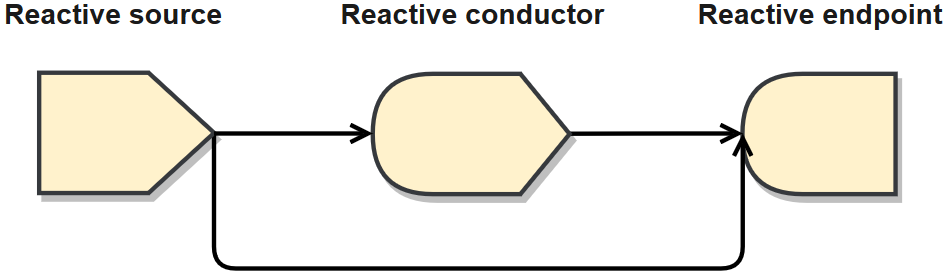
\includegraphics[width=0.7\linewidth]{Imagens/reactive}
	\caption{Representation of reactive programming objects in a Shiny application.}
	\label{reactive}
\end{figure}

The reactive source typically consists in the user input through a browser interface (e.g. selecting an item, typing input). A reactive endpoint is usually something that appears in the user's browser window, such as a plot or a table of values. A reactive source can be connected to multiple endpoints, and vice versa. Most simple examples use just these two components, wiring up sources directly to endpoints. However, it is also possible to put reactive components between the sources and endpoints, namely reactive conductors. These can be useful for encapsulating slow or computationally expensive operations, making sure code does not run more times than the absolutely necessary.

Other R libraries were also used. These include:
%the \textit{shinydashboard} library that allows the construction of a shiny application with a typical dashboard appearance; \textit{shinyBS} which adds additional Twitter Bootstrap components to Shiny including, for instance, modal windows; \textit{shinyjs} that allows to perform common useful JavaScript operations in Shiny apps like hiding, reseting or disabling elements; the \textit{DT} library that allows data objects in R to be rendered as HTML tables; \textit{RMySQL} library which is a database interface to MySQL; \textit{bcrypt} library for string encryption (used for the authentication system); the \textit{GGally} which is an extension of the graphics package \textit{ggplot2}; \textit{shinyWidgets} library that adds better looking custom inputs widgets to shiny applications; and the \textit{colourpicker} library that has a colour picker that can be used as an input in a shiny application, useful for interactively changing the color of some plots, for instance.

\begin{itemize}
	\item \textit{\textbf{shinydashboard}}: allows the construction of a shiny application with a typical dashboard appearance;
	\item \textit{\textbf{shinyBS}}: adds additional Twitter Bootstrap components to Shiny including, for instance, modal windows;
	\item \textit{\textbf{shinyjs}}: allows to perform common useful JavaScript operations in Shiny apps like hiding, reseting or disabling elements;
	\item \textit{\textbf{DT}}: allows data objects in R to be rendered as HTML tables;
	\item \textit{\textbf{RMySQL}}: a database interface to MySQL;
	\item \textit{\textbf{bcrypt}}: for string encryption (used for the authentication system);
	\item \textit{\textbf{GGally}}:	an extension of the graphics package \textit{ggplot2};
	\item \textit{\textbf{shinyWidgets}}: adds better looking custom inputs widgets to shiny applications;	
	\item \textit{\textbf{colourpicker}}: has a colour picker that can be used as an input in a shiny application, useful for interactively changing the color of some plots, for instance.
\end{itemize}

More importantly, the \textit{specmine} package was used, providing a set of methods for me\-ta\-bo\-lo\-mics data analysis, including data loading in different formats, pre-processing, metabolite identification, univariate and multivariate data analysis, machine learning and feature selection. The package functionalities will be introduced in detail in the next section, given its importance for this work.

The \gls{ide} chosen to develop the R scripts and build the platform was RStudio (\href{https://www.rstudio.com/}{\nolinkurl{https://www.rstudio.com/}}). It is written in the C++ programming language, having an intuitive interface with many usefull tools, making it easier to work with R. RStudio is a free software that has many features, including a console, syntax-highlighting editor that supports direct code execution, as well as tools for plotting, history, debugging and workspace management. 

Reports with the analysis results generated on the platform were made using the RStudio plug-in named R Markdown (\href{http://rmarkdown.rstudio.com/}{\nolinkurl{http://rmarkdown.rstudio.com/}}). R Markdown uses markdown syntax (\href{https://daringfireball.net/projects/markdown/}{\nolinkurl{https://daringfireball.net/projects/markdown/}}) coupled with R code chunks that are run, displaying the code's output in the generated report. The report is generated using the \textit{knitr} package (\href{https://yihui.name/knitr/}{\nolinkurl{https://yihui.name/knitr/}}), the engine for dynamic report generation with R, and it can be in the form of a HTML, PDF or Microsoft Word document. 

The database for project, dataset and user management was built using the open-source \gls{rdbms} MySQL (\href{https://www.mysql.com/}{\nolinkurl{https://www.mysql.com/}}). It is written in C and C++, being a fast, stable and multi-user, multi-threaded \gls{sql} database server. \gls{sql} consists of a data definition, manipulation and control language. It is a special-purpose domain-specific language used in programming and designed for stream processing or managing data held in a \gls{rdbms}. The scope of \gls{sql} includes data insert, query, update and delete, schema creation and modification, and data access control. 




